\section{Introduction}
Security operations centers must turn many detector outputs into a smaller number of reviewable incidents. Aggregation can reduce an analyst's workload, but a plausible relationship is not necessarily a trustworthy relationship: a copied claim may look like an independent witness, an event timestamp may precede the time its evidence became available, and a shared host or account may join unrelated activity. Research on domain-independent aggregation, multi-stage reconstruction, and triage addresses different parts of this problem \cite{landauer2022,wang2024,grain2025,sadlek2025}. The safety of a reconstructed incident depends on the evidence that justifies each cross-fragment union.

We study a specific decision problem: at a fixed cutoff, partition the alerts that have become visible into incident candidates, while refusing a cross-fragment link when its attestation is unavailable, dependent, inconsistent, or contradicted. The resulting groups are ranked for analyst review. Correlation proposes relationships; verification controls which extra unions can occur; ranking cannot repair a missing group. Prior work often emphasizes alert reduction, attack prediction, graph reconstruction, or prioritization, and these objectives and their labels are not interchangeable \cite{malach2025,grain2025,chuah2025}.
Figure~\ref{fig:arch} previews the implemented pipeline and the distinct responsibilities of correlation, verification, and prioritization.
\begin{figure*}[t]\centering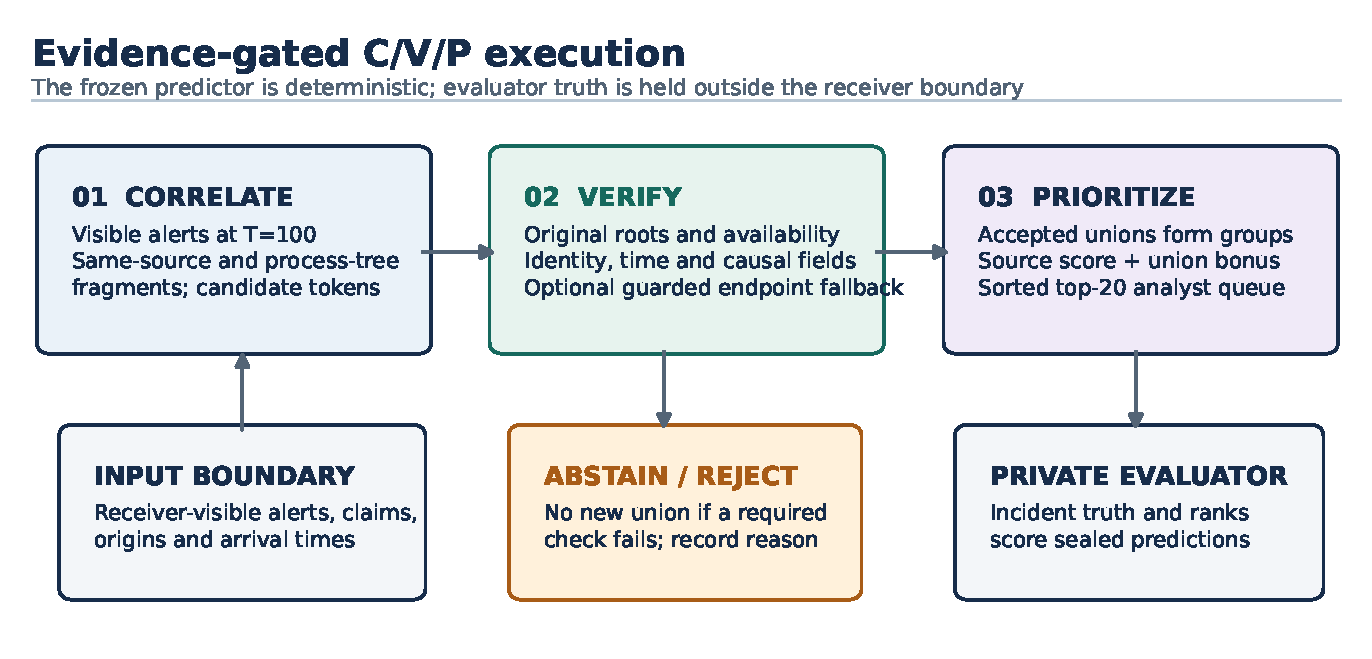
\includegraphics[width=.86\textwidth]{figures/architecture.pdf}\caption{Implemented C/V/P architecture. Receiver-visible alerts and claims enter initial correlation (C); independent-root, identity and temporal verification (V) controls additional fragment unions; prioritization (P) ranks the final groups. Rejected or insufficient bundles do not add a union. Private evaluator labels never enter prediction.}\label{fig:arch}\end{figure*}

Our questions are: (RQ1) how does the implemented provenance and point-in-time verifier constrain cross-fragment reconstruction under incomplete evidence; (RQ2) does an endpoint-based fallback improve recoverability and retrieval on a matched, untouched synthetic holdout without observed unsafe unions; and (RQ3) what evidence limits further ranking gains and a valid external test? The contributions are:
\begin{itemize}
\item a bounded C/P/V role architecture and an exact description of the implemented deterministic verification path;
\item a matched fresh synthetic holdout with incident, ranking, grouping and token-decision metrics, including negative queue outcomes;
\item a cross-track audit that separates retrospective GUIDE and bounded LLM work from the synthetic result, and a concrete external-validation protocol.
\end{itemize}
No superiority over published systems on incompatible datasets is claimed. The remainder moves from related work and methodology through experiments, base-paper comparison, ablation and limitations to conclusions and declarations.
